% Options for packages loaded elsewhere
\PassOptionsToPackage{unicode}{hyperref}
\PassOptionsToPackage{hyphens}{url}
%
\documentclass[ignorenonframetext,aspectratio=169]{beamer}

\usepackage{pgfpages}

\setbeamertemplate{caption}[numbered]
\setbeamertemplate{caption label separator}{: }
\setbeamercolor{caption name}{fg=normal text.fg}
\beamertemplatenavigationsymbolsempty

% Prevent slide breaks in the middle of a paragraph
\widowpenalties 1 10000
\raggedbottom
\setbeamertemplate{part page}{
  \centering
  \begin{beamercolorbox}[sep=16pt,center]{part title}
    \usebeamerfont{part title}\insertpart\par
  \end{beamercolorbox}
}
\setbeamertemplate{section page}{
  \centering
  \begin{beamercolorbox}[sep=12pt,center]{part title}
    \usebeamerfont{section title}\insertsection\par
  \end{beamercolorbox}
}
\setbeamertemplate{subsection page}{
  \centering
  \begin{beamercolorbox}[sep=8pt,center]{part title}
    \usebeamerfont{subsection title}\insertsubsection\par
  \end{beamercolorbox}
}
\AtBeginPart{
  \frame{\partpage}
}
\AtBeginSection{
  \ifbibliography
  \else
    \frame{\sectionpage}
  \fi
}
\AtBeginSubsection{
  \frame{\subsectionpage}
}

\usepackage{amsmath,amssymb}
\usepackage{iftex}
\ifPDFTeX
  \usepackage[T1]{fontenc}
  \usepackage[utf8]{inputenc}
  \usepackage{textcomp} % provide euro and other symbols
\else % if luatex or xetex
  \usepackage{unicode-math}
  \defaultfontfeatures{Scale=MatchLowercase}
  \defaultfontfeatures[\rmfamily]{Ligatures=TeX,Scale=1}
\fi

\usepackage{lmodern}
\ifPDFTeX\else  
    % xetex/luatex font selection
\fi

% Use upquote if available, for straight quotes in verbatim environments
\IfFileExists{upquote.sty}{\usepackage{upquote}}{}
\IfFileExists{microtype.sty}{% use microtype if available
  \usepackage[]{microtype}
  \UseMicrotypeSet[protrusion]{basicmath} % disable protrusion for tt fonts
}{}
\makeatletter
\@ifundefined{KOMAClassName}{% if non-KOMA class
  \IfFileExists{parskip.sty}{%
    \usepackage{parskip}
  }{% else
    \setlength{\parindent}{0pt}
    \setlength{\parskip}{6pt plus 2pt minus 1pt}}
}{% if KOMA class
  \KOMAoptions{parskip=half}}
\makeatother
\usepackage{xcolor}
\newif\ifbibliography
\setlength{\emergencystretch}{3em} % prevent overfull lines
\setcounter{secnumdepth}{-\maxdimen} % remove section numbering


\providecommand{\tightlist}{%
  \setlength{\itemsep}{0pt}\setlength{\parskip}{0pt}}\usepackage{longtable,booktabs,array}
\usepackage{calc} % for calculating minipage widths
\usepackage{caption}
% Make caption package work with longtable
\makeatletter
\def\fnum@table{\tablename~\thetable}
\makeatother
\usepackage{graphicx}
\makeatletter
\def\maxwidth{\ifdim\Gin@nat@width>\linewidth\linewidth\else\Gin@nat@width\fi}
\def\maxheight{\ifdim\Gin@nat@height>\textheight\textheight\else\Gin@nat@height\fi}
\makeatother
% Scale images if necessary, so that they will not overflow the page
% margins by default, and it is still possible to overwrite the defaults
% using explicit options in \includegraphics[width, height, ...]{}
\setkeys{Gin}{width=\maxwidth,height=\maxheight,keepaspectratio}
% Set default figure placement to htbp
\makeatletter
\def\fps@figure{htbp}
\makeatother

\makeatletter
\makeatother
\makeatletter
\makeatother
\makeatletter
\@ifpackageloaded{caption}{}{\usepackage{caption}}
\AtBeginDocument{%
\ifdefined\contentsname
  \renewcommand*\contentsname{Daftar Isi}
\else
  \newcommand\contentsname{Daftar Isi}
\fi
\ifdefined\listfigurename
  \renewcommand*\listfigurename{Daftar Gambar}
\else
  \newcommand\listfigurename{Daftar Gambar}
\fi
\ifdefined\listtablename
  \renewcommand*\listtablename{Daftar Tabel}
\else
  \newcommand\listtablename{Daftar Tabel}
\fi
\ifdefined\figurename
  \renewcommand*\figurename{Gambar}
\else
  \newcommand\figurename{Gambar}
\fi
\ifdefined\tablename
  \renewcommand*\tablename{Tabel}
\else
  \newcommand\tablename{Tabel}
\fi
}
\@ifpackageloaded{float}{}{\usepackage{float}}
\floatstyle{ruled}
\@ifundefined{c@chapter}{\newfloat{codelisting}{h}{lop}}{\newfloat{codelisting}{h}{lop}[chapter]}
\floatname{codelisting}{Daftar}
\newcommand*\listoflistings{\listof{codelisting}{Daftar Daftar}}
\makeatother
\makeatletter
\@ifpackageloaded{caption}{}{\usepackage{caption}}
\@ifpackageloaded{subcaption}{}{\usepackage{subcaption}}
\makeatother
\makeatletter
\@ifpackageloaded{tcolorbox}{}{\usepackage[skins,breakable]{tcolorbox}}
\makeatother
\makeatletter
\@ifundefined{shadecolor}{\definecolor{shadecolor}{rgb}{.97, .97, .97}}
\makeatother
\makeatletter
\makeatother
\makeatletter
\makeatother

\ifLuaTeX
\usepackage[bidi=basic]{babel}
\else
\usepackage[bidi=default]{babel}
\fi
\babelprovide[main,import]{indonesian}

% get rid of language-specific shorthands (see #6817):
\let\LanguageShortHands\languageshorthands
\def\languageshorthands#1{}

\ifLuaTeX
  \usepackage{selnolig}  % disable illegal ligatures
\fi

\IfFileExists{bookmark.sty}{\usepackage{bookmark}}{\usepackage{hyperref}}
\IfFileExists{xurl.sty}{\usepackage{xurl}}{} % add URL line breaks if available
\urlstyle{same} % disable monospaced font for URLs

\usepackage{minted}

\newminted{julia}{breaklines,fontsize=\footnotesize}
\newminted{python}{breaklines,fontsize=\footnotesize}

\newminted{bash}{breaklines,fontsize=\footnotesize}
\newminted{text}{breaklines,fontsize=\footnotesize}

\newcommand{\txtinline}[1]{\mintinline[breaklines,fontsize=\footnotesize]{text}{#1}}
\newcommand{\jlinline}[1]{\mintinline[breaklines,fontsize=\footnotesize]{julia}{#1}}
\newcommand{\pyinline}[1]{\mintinline[breaklines,fontsize=\footnotesize]{python}{#1}}



\title{TF2202: Pendahuluan}
\author{Fadjar Fathurrahman}
\date{}

\begin{document}

\frame{\titlepage}
\ifdefined\Shaded\renewenvironment{Shaded}{\begin{tcolorbox}[enhanced, borderline west={3pt}{0pt}{shadecolor}, interior hidden, sharp corners, boxrule=0pt, frame hidden, breakable]}{\end{tcolorbox}}\fi

\begin{frame}{Sekilas mengenai kuliah ini}
\protect\hypertarget{sekilas-mengenai-kuliah-ini}{}
\begin{itemize}
\item
  Kode dan nama kuliah: Komputasi Rekayasa
\item
  Nama lain: metode numerik, komputasi teknik
\item
  Dalam kuliah ini kita akan mempelajari \emph{metode-metode numerik}
  yang diimplementasikan dengan menggunakan komputer dengan aplikasi
  yang sesuai dan/atau bahasa pemrograman. Metode-metode numerik ini
  akan digunakan untuk menyelesaikan \emph{persamaan matematis} yang
  muncul pada pemodelan masalah yang muncul pada sains dan keteknikan.
\end{itemize}
\end{frame}

\begin{frame}{Sekilas mengenai kuliah ini}
\protect\hypertarget{sekilas-mengenai-kuliah-ini-1}{}
\begin{itemize}
\item
  Beban: 3 SKS
\item
  Referensi:

  \begin{itemize}
  \tightlist
  \item
    S. C. Chapra and R. P. Canale. Numerical Methods for Engineers. (7th
    Ed)
  \end{itemize}
\end{itemize}
\end{frame}

\begin{frame}{Apa yang akan dipelajari}
\protect\hypertarget{apa-yang-akan-dipelajari}{}
\begin{itemize}
\item
  Aproksimasi dan galat
\item
  Pencarian akar
\end{itemize}
\end{frame}




\begin{frame}{Tools yang akan digunakan}

Ada beberapa tools yang dapat kita gunakan:
\begin{itemize}
\item Python, Julia, MATLAB, Fortran, \emph{spreadsheet}
\end{itemize}

\end{frame}




\begin{frame}{Contoh: \emph{bungee jumper}}

\fontsize{9pt}{10pt}\selectfont

\begin{columns}

\begin{column}{0.2\textwidth}

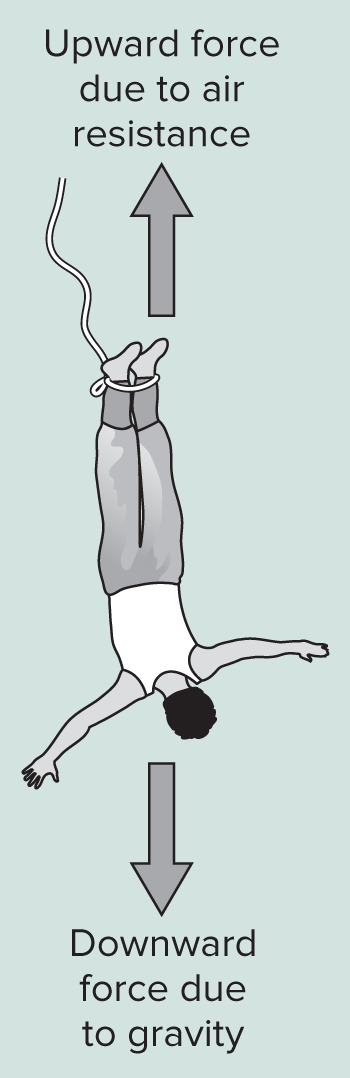
\includegraphics[height=0.7\textheight]{../images_priv/Chapra_Fig_1_1.png}

\end{column}

\begin{column}{0.8\textwidth}
Misalkan kita diminta untuk menghitung kecepatan $v(t)$ dari pelompat
\emph{bungee} yang sedang terjun. Untuk mendapatkan ini, kita
menggunakan Hukum Newton:
\begin{equation*}
F = m \frac{\mathrm{d}}{\mathrm{d}t} v(t)
\end{equation*}
dengan $F$ adalah gaya total dan $m$ adalah massa pelompat.
Gaya yang bekerja pada penerjun ada dua, yaitu gaya gravitasi \(F_{g}\) dan
gaya akibat gesekan udara (\emph{drag})
$F_{d}$:
\begin{equation*}
F = F_{g} + F_{d}
\end{equation*}
dengan: $F_{g} = mg$, dengan $g$ adalah percepatan gravitasi dan gaya
gesekan diudara diasumsikan berbanding lurus dengan kecepatan:
\begin{equation*}
F_{d} = -c v  
\end{equation*}
dengan $c$ adalah suatu konstanta.
\end{column}

\end{columns}

\end{frame}


\begin{frame}{Contoh: \emph{bungee jumper}}

Sehingga dapat diperoleh persamaan gerak untuk \emph{bungee jumper}:
\begin{equation}
\frac{\mathrm{d}v}{\mathrm{d}t} = g - \frac{c}{m}v
\label{eq:diff-eq-01}
\end{equation}

Bagaimana cara menyelesaikan persamaan diferensial ini? Kita dapat
menggunakan kalkulus untuk mencari solusi analitiknya. Dengan
menggunakan informasi tambahan (syarat awal) bahwa $v(t=0)=0$, dapat
diperoleh solusi analitik:
\begin{equation}
v(t) = \frac{gm}{c}\left( 1 - e^{(c/m)t} \right)
\label{eq:sol-diff-eq-01}
\end{equation}
Untuk verifikasi bahwa
persamaan ini merupakan solusi substitusi
Pers. \eqref{eq:sol-diff-eq-01} ke Pers. \eqref{eq:diff-eq-01}
\end{frame}



\begin{frame}{Solusi analitik}

\fontsize{9pt}{10pt}\selectfont

Dengan menggunakan nilai-nilai berikut: $m = 68.1$ kg, $g = 9.81$
$\mathrm{m}/\mathrm{s}^2$, $c = 12.5$ kg/s
kita dapat menghitung kecepatan sebagai fungsi dari waktu $t$.
Contoh dapat dilihat pada tabel berikut.

{\centering
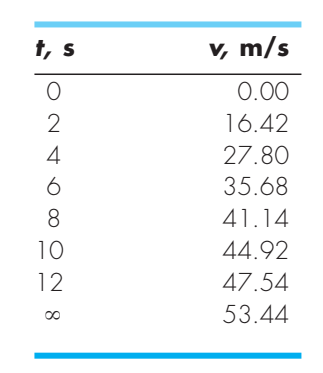
\includegraphics[height=0.5\textheight]{../chapra_7th/Chapra_Example_1_1_table.png}
\par}

Kecepatan pada $t \rightarrow \infty$ dikenal juga sebagai kecepatan akhir
(\emph{terminal velocity}).

TUGAS: Tulis program Python untuk membuat plot dari $v(t)$ terhadap $t$.

\end{frame}



\begin{frame}{Solusi numerik}
Solusi yang baru saja kita dapatkan adalah solusi eksak atau solusi
analitik.

Bagaimana jika:

\begin{itemize}\tightlist
\item kita lupa cara mengintegralkan atau menyelesaikan persamaan
  diferensial yang diperoleh?
\item persamaan diferensial yang diperoleh rumit sehingga tidak ada
  solusi analitik yang tersedia
\end{itemize}

Alternatif yang dapat kita gunakan adalah dengan menggunakan
\emph{metode numerik}.
\end{frame}



\begin{frame}{Aproksimasi dan Metode numerik}

\begin{columns}[T]
\begin{column}{0.5\textwidth}
{\centering
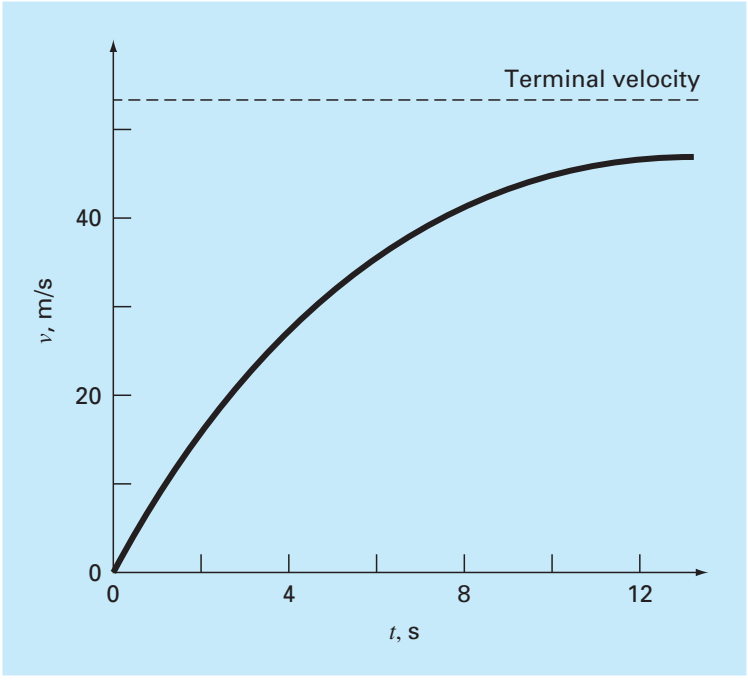
\includegraphics[width=1\textwidth,height=\textheight]{../images_priv/Chapra_Fig_1_3.png}
\par}
\end{column}

\begin{column}{0.5\textwidth}
Dengan menggunakan metode numerik, kita dapat mengaproksimasi turunan
dengan menggunakan:
\begin{equation*}
\frac{\mathrm{d}v}{\mathrm{d}t} \approx \frac{v_{i+1} - v_{i}}{t_{i+1} - t_{i}}
\end{equation*}

Perhatikan bahwa kita telah \emph{mendiskritisasi} kecepatan \(v(t)\)
dan waktu \(t\) pada persamaan di atas, artinya \(v\) dan \(t\) tidak
lagi memiliki nilai yang kontinu, namun diskrit, seperti pada nilai
dalam tabel. Solusi numerik yang akan kita dapatkan hanya tersedia pada
titik-titik diskrit tersebut.
\end{column}
\end{columns}
\end{frame}




\begin{frame}{Solusi numerik}

\fontsize{9pt}{10pt}\selectfont

Pers. \eqref{eq:diff-eq-01} dapat
diaproksimasi menjadi:
\begin{equation*}
\frac{v_{i+1} - v_{i}}{t_{i+1} - t_{i}} = g - \frac{c}{m} v_{i}
\end{equation*}

\begin{equation*}
v_{i+1} = v_{i} + \underbrace{\left( g - \frac{c}{m} v_{i} \right)}_{
  \left.\dfrac{\mathrm{d}v}{\mathrm{d}x}\right|_{t_{i},v_{i}}
}
\underbrace{\left( t_{i+1} - t_{i} \right)}_{\Delta t}
\end{equation*}

Metode ini juga dapat dinyatakan dengan deskripsi berikut:
\begin{equation*}
\text{nilai baru} = \text{nilai lama} + \text{kemiringan}\times\text{ukuran langkah}
\end{equation*}
Metode ini dikenal dengan \emph{metode Euler}. Kita akan mempelajari
lebih lanjut mengenai metode ini pada bab mengenai persamaan diferensial
(persoalan nilai awal).
\end{frame}



\begin{frame}{Solusi numerik}

\begin{columns}[T]
\begin{column}{0.5\textwidth}
Dengan menggunakan ukuran langkah \(\Delta t = 2\) s, \(t_0 = 0\),
\(v_0 = 0\) kita dapat menghitung: \[
v_1 = 0 + \left[ 9.81 - \frac{12.5}{68.1}(0) \right] 2 = 19.62
\]

\[
v_2 = 19.62 + \left[ 9.81 - \frac{12.5}{68.1}(19.62) \right] 2 = 32.04
\]
\end{column}

\begin{column}{0.5\textwidth}

Dengan meneruskan perhitungan ini dapat diperoleh tabel berikut.

{\centering
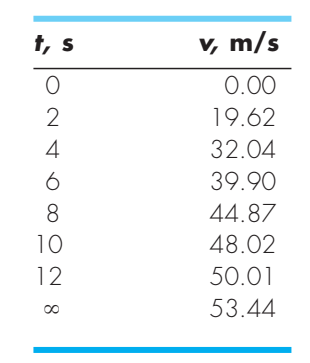
\includegraphics[width=\textwidth,height=0.5\textheight]{../chapra_7th/Chapra_Example_1_2_table.png}
\par}

\end{column}

\end{columns}

\end{frame}



\begin{frame}{Solusi analitik vs solusi numerik}

{\centering
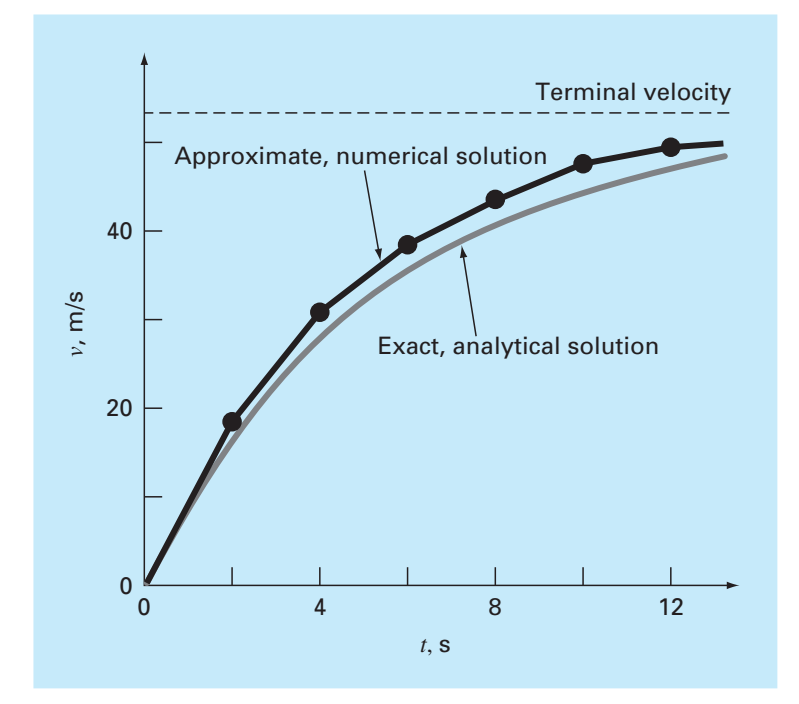
\includegraphics[height=0.8\textheight]{../chapra_7th/Chapra_Fig_1_5.png}
\par}

\end{frame}



\begin{frame}{Langkah-langkah penyelesaian masalah}

\begin{enumerate}
[(1)]
\item
  Identifikasi permasalahan
\item
  Pemodelan: hukum fisika, asumsi dan aproksimasi fisis penurunan
  persamaan matematika
\item
  Aproksimasi numerik, penurunan persamaan diskrit
\item
  Implementasi pada komputer (menggunakan perangkat lunak khusus atau
  dengan menulis program) untuk mendapatkan solusi
\item
  Visualisasi solusi
\item
  Analisis (termasuk validasi dan verifikasi)
\end{enumerate}

Pada kuliah ini kita akan lebih fokus pada Langkah (3), (4) dan (5)
\end{frame}




\begin{frame}{Tugas}

Ulangi kasus untuk peloncat \emph{bungee} pada contoh sebelumnya, jika
sekarang gaya gesekan yang bekerja berbanding lurus dengan \emph{kuadrat
kecepatan} \[
F_{d} = c v^2
\] dengan \(c_d\) adalah koefisien gesekan. Bandingkan solusi numerik
yang Anda dapatkan dengan solusi analitik \[
v(t) = \sqrt{\frac{g m}{c}}\tanh\left( \frac{g c}{m} t \right)
\]
\end{frame}



\end{document}
